\section{}
A thin plate moves between two parallel, horizontal, stationary flat 
surfaces at a constant velocity of 5 m/s as shown in the figure. The two 
stationary surfaces are spaced 4 cm apart, and the medium between them is 
filled with oil whose viscosity is 0.9 N $\cdot$ s/m$^2$. The part of the
plate immersed in oil at any given time is 2-m long and 0.5-m wide. If the
plate moves through the mid-plane between the surfaces, determine the force
required to maintain this motion. What would your response be if the plate
was 1 cm from the bottom surface ($h_2$) and 3 cm from the top surface ($h_1$)?

\begin{figure}[h]
    \centering
    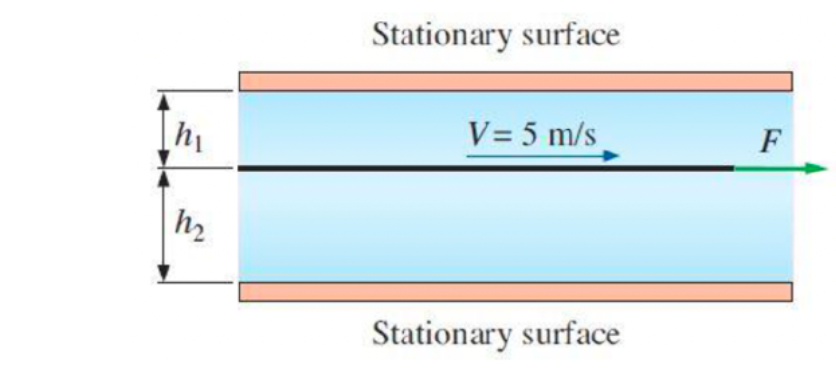
\includegraphics[width=0.5\textwidth]{Questions/Figures/Q1ProblemDiagram.png}
    \caption{Plate moving between two parallel surfaces.}
    \label{fig:Q1ProblemDiagram}
\end{figure}

\subsection{}
\textit{The plate moves through the mid-plane between the surfaces.}

Assumptions:
\begin{itemize}
    \item Oil is a Newtonian fluid
    \item The velocity profile is linear
\end{itemize}

Since the velocity profile is linear, the shear stress can be calculated using
the following equation:
\begin{equation}
    \tau = \mu \frac{du}{dy}
    \label{eq:ShearStress}
\end{equation}

\begin{figure}[h]
    \centering
    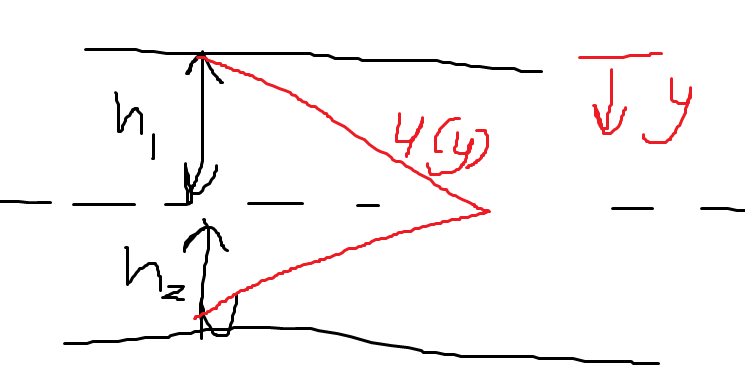
\includegraphics[width=0.5\textwidth]{Questions/Figures/Q1LinearVelocityProfile.png}
    \caption{Velocity profile for Question 1.}
    \label{fig:Q1VelocityProfile}
\end{figure}

The velocity as a function of $y$ is:
\begin{align}
    u(y) &= \frac{u_{max}}{h_1}y \label{eq:LinearVelocityProfile} \\
    \frac{du}{dy} &= \frac{u_{max}}{h_1} \label{eq:LinearVelocityProfileDerivative}
\end{align}

Substituting Equation (\ref{eq:LinearVelocityProfileDerivative}) into Equation
(\ref{eq:ShearStress}) yields:
\begin{align}
    \tau_{top} &= \mu \frac{u_{max}}{h_1} \nonumber \\
        &= 0.9 \frac{5}{0.02} \nonumber \\
        &= \qty{225}{N/m^2} \nonumber
\end{align}

Similarly, $\tau_{bottom} = \qty{225}{N/m^2}$.

The force required to maintain the motion is:
\begin{align}
    F &= \tau_{top} A \nonumber \\
        &= 225 \cdot 2 \cdot 0.5 \nonumber \\
        &= 225 \unit{N} \nonumber
\end{align}

By symmetry, the force required to maintain the motion is the same for the
bottom surface. Therefore,

\begin{equation*}
    \boxed{F = \qty{450}{\newton}}
\end{equation*}

\subsection{}
\textit{The plate is 1 cm from the bottom surface ($h_2$) and 3 cm from the top surface ($h_1$).}

By similar methods,
\begin{align*}
    F = F_{top} + F_{bottom} &= \tau_{top} A + \tau_{bottom} A \\
        &= \mu A \left(\frac{u_{max}}{h_1} + \frac{u_{max}}{h_2}\right) \\
        &= 0.9 \cdot 2 \cdot 0.5 \left(\frac{5}{0.03} + \frac{5}{0.01}\right) \\
        &= 0.9(166.67 + 500) \\
        &= \boxed{\qty{600}{\newton}}
\end{align*}